%%%%%%%%%%%%%%%%%%%%%%%%%%%%%%%%%%%%%%%%%%%%%%%%%%%%%%%%%%%%%%%%%%%%%%%%%%%%%%%
\section{Review of discretizations for polygonal meshes} \label{sec_review}
%%%%%%%%%%%%%%%%%%%%%%%%%%%%%%%%%%%%%%%%%%%%%%%%%%%%%%%%%%%%%%%%%%%%%%%%%%%%%%%

In this Section, we review different discretizations that can be used on polygonal
meshes.

%-----------------------------------------------------------
\subsection{Palmer's method}
%-----------------------------------------------------------

Palmer's method is a node- or point-based method \cite{Palmer2001}. This
discretization is second order and uses a finite volume approach: the
particle balance is enforced by integrating over a control volume. The control 
volume is the union of all corners surrounding a vertex $p$. A corner is a
quadrilateral defined by the vertex $p$, the cell-center $c$, and the midpoint
of the edges $e$ that contain the point $p$. On a triangular grid, the
scheme is equivalent to linear continuous finite elements with ``mass-matrix
lumping''. This method works for any, even concave, polygonal cell. The
main disadvantage of Palmer's method is that the discretization of the
diffusion equation does not lead to symmetric system in the general case.

%-----------------------------------------------------------
\subsection{Mimetic finite differences}
%-----------------------------------------------------------
Mimetic methods, such as mimetic finite differences (MFD), mimic properties of
mathematical and physical models, such as: tensor and vector calculus,
conservation laws, symmetry preservation, solution positivity and
monotonicity, and asymptotic limits (e.g., diffusion limit), on polygonal and
polyhedral meshes. The most important part of MFD is the definition of a scalar
product which satisfies stability and consistency some conditions
\cite{Brezzi2005}. However, this scalar product is not unique and therefore,
multiple MFD methods exists. MFD is efficient even on concave polygons
\cite{Kuznetsov2004}. MFD methods are related to mixed finite elements.

%\red{An important (mimetic) property of operators div and $K\bn$ is expressed
%  by integration by part formula:
%  \begin{equation}
%    \int_{\bo} K^{-1}\bs{u} \cdot (K\bn p)dV = - \int_{\bo} (div\ \bs{u}) p\ dV
%  \end{equation}
%  which holds for any $p \in H_0^1(\bo)$ and $\bs{u}\in H_{div}(\bo)$.\\
%  The MFD method mimics this property by replacing integrals and operators by
%  their discrete counterparts:
%  \begin{equation}
%    [\bs{U},GRAD\ P]_X = -[DIV\ \bs{U},P]_Q
%  \end{equation}
%which holds for any vectors of degrees of freedom $P$ and $\bs{U}$. MFD
%connected to mixed finite elements. Works with mixed cells.}
%\red{Mimetic numerical methods mimic crucial properties of mathematical and
%  physical models on arbitrary on polygonal and polyhedral meshes:
%  \begin{itemize}
%    \item tensor and vector calculus
%    \item conservation laws
%    \item symmetry preservation
%    \item solution positivity and monotonicity
%    \item asymptotic limits (e.g., diffusion limit in radiation transport
%      models)
%  \end{itemize}}
%\red{\cite{Lipnikov2004} only quadrilaterals with at most one hanging node per edge. 
%  SO can be applied to many forms of the diffusion equation, but here we consider
%the first-order form of the diffusion equation. Use local SO.
%\begin{itemize}
%  \item there are two different support-operators methods, they both
%        give the same cell-center intensity solutions:
%    \begin{itemize}
%      \item one has intensity unknowns located only at cell centers: the
%        diffusion matrix is dense.
%      \item one has intensity unknowns located at both cell centers and face
%        centers: the diffusion matrix is space. The cell-center unknowns are
%        locally eliminated, resulting in a reduced system consisting only of
%        the face-center unknowns. The method is called the local SO method.
%    \end{itemize}
%  \item local SO is composed of two steps:
%    \begin{itemize}
%      \item consider each cell in the domain as a independent domain and
%        generate an independent discretization for each cell (identical to
%        what is done for standard quadrilateral meshes)
%      \item obtain a global discretization by imposing continuity of the
%        intensity and continuity of the normal component of the flux across
%        cell interfaces. 
%    \end{itemize}
%\end{itemize}
%\cite{Hyman2002} the mimetic FDM are based on discrete of first-order
%coordinate-invariant operators, it is natural to write the diffusion equation
%as a system of first order equations.
%\cite{Kuznetsov2004} works for any polygons. Used in geophysics $->$ the equation is
%split in two first-order equations.
%\begin{itemize}
%  \item exact for linear solution
%  \item SPD
%\end{itemize}
%\cite{Brezzi2005} the key element of the MFD method is the scalar product in the
%space of discrete velocities which should satisfy the stability assumption and
%the consistency assumption. It turns out that such a scalar product is not
%unique.
%\begin{enumerate}
%  \item specify the degrees of freedom for the primary variables
%  \item define suitable scalar products in the discrete spaces
%  \item discretize the divergence operator
%  \item define the discrete flux operator
%\end{enumerate}}

%-----------------------------------------------------------
\subsection{Wachspress' rationale finite element}
%-----------------------------------------------------------
Before introducing the Wachspress' basis function on a quadrilateral cell, 
we define $P_{1,2}(x,y)$ the polynomial defined by the points $(x_1,y_1)$ and
$(x_2,y_2)$:
\begin{equation}
  P_{1,2}(x,y) = (y-y_1) (x_2-x_1)-(x-x_1)(y_2-y_1).
\end{equation}  
Using this definition, Wachspress' basis functions are given by:
\begin{align}
  &b_0(x,y) = k_0 P_{2,3}(x,y)P_{1,2}(x,y)/P_{4,5}(x,y),\\
  &b_1(x,y) = k_1 P_{0,3}(x,y)P_{2,3}(x,y)/P_{4,5}(x,y),\\
  &b_2(x,y) = k_2 P_{0,1}(x,y)P_{3,0}(x,y)/P_{4,5}(x,y),\\
  &b_3(x,y) = k_3 P_{1,2}(x,y)P_{0,1}(x,y)/P_{4,5}(x,y),
\end{align}
where $k_i$ are chosen such that $b_i(x_i,y_i)=1$. $(x_4,y_4)$ and $(x_5,y_5)$
are the intersections of the prolongations of the edges 
of the quadrilaterals (see \Cref{fig_quadrilateral}).
\begin{figure}[H]
  \centering
  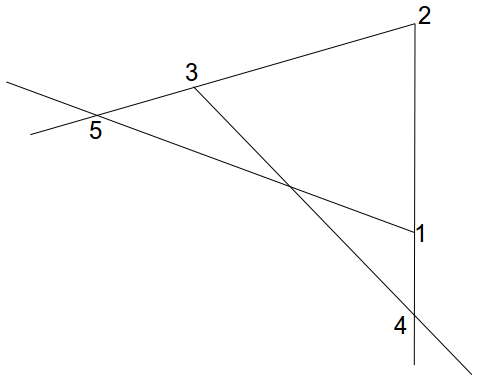
\includegraphics[width=5cm]{quadrilateral}
  \caption{Quadrilateral cell}
  \label{fig_quadrilateral}
\end{figure}
These two points uniquely defines a linear polynomial. It should be noted that 
the line defined by $(x_4,y_4)$ and $(x_5,y_5)$ does not pass through the 
quadrilateral and thus, the denominator cannot vanish (this is 
only true for convex quadrilateral). When the quadrilateral tends to a 
parallelogram, the points defining $P_{4,5}$ are moved to infinity and 
$P_{4,5}(x,y)$ tends to a constant inside the quadrilateral. By definition, 
this constant is chosen to be one for a parallelogram. For a trapezoid,
$P_{4,5}(x,y)=0$ is the equation of the line parallel to the two parallel
edges of the trapezoid which contains the intersection of the prolongations of
the two non-parallel edges. For arbitrary polygons, a non-trivial 
generalization is necessary \cite{Wachspress1975}.
%\red{\cite{Bailey2008a} he disadvantage is that the basis function integrals must
%be done numerically.
%\red{\cite{Wachspress1975} $(r;q)_2|_3$ is the value at point 3 of a quadratic
%  function containing points $r$ and $q$. This value depends on supplementary
%  data which defines the quadratic function $(r;q)_2$. Similarly
%  $[(1;2)_2(3;4)/(1;5)]|_8$ is the value of the indicated rational function
%  at point 8. For quadrilaterals: we look for a function like:
%  \begin{equation}
%    w_1(x,y) = \frac{Q_1}{(2;3)(3;4)}|_1 \frac{(2;3)(3;4)}{Q_1}
%  \end{equation}
%  We therefore seek a linear from $Q_1$ such that:
%  \begin{itemize}
%    \item $Q_1\neq 0$ within the quadrilateral
%    \item $\frac{(2;3)(3;4}{Q_1}$ is linear on both $(4;1)$ and $(1;2)$
%  \end{itemize}
%  The first property has far-reaching consequences: we must broaden our vision
%  and look outside the quadrilateral. We observe that all the linear forms
%  appearing in the triangle and parallelogram wedges were determined by the
%  sides of these figures. We shall soon see that the quadrilateral itself
%  reaches out to give us the desired linear form. First, we need the following
%  lemma: \emph{If three lines intersect at a point then the ratio of linear
%  forms which vanish on any two of these lines is constant on the third line.}
%  We choose $Q_1$ so that $(2;3)/Q_1$ is constant on side $(4;1)$ and so that
%  $(3;4)/Q_1$ is constant on side $(4;1)$ and so that $(3;4)/Q_1$ is constant
%  on side $(1;2)$. By the lemma, the first requirement is met if lines
%  $(2;3)$, $(4;1)$, and $Q_1$ have a common point of intersection and the
%  second requirement is met if lines $(3;4)$, $(1;2)$, and $Q_1$ have a common
%  point of intersection. If we define point 5 as the intersection point of
%  lines $(2;3)$ and $(1;4)$ and point 6 as the intersection of $(1;2)$ and
%  $(3;4)$, we find that $Q_1(x,y) = (5;6)$ is the unique line which meets both
%  requirements. For any convex quadrilateral, line $Q_1$ has no point in the
%  quadrilateral. Consistent candidates for all four wedges are:
%  \begin{subequations}
%    \begin{align}
%      &W_1(x,y) = k_1 (2;3)(3;4)/Q_1(x,y)\\
%      &W_2(x,y) = k_2 (3;4)(4;1)/Q_1(x,y)\\
%      &W_3(x,y) = k_3 (4;1)(1;2)/Q_1(x,y)\\
%      &W_4(x,y) = k_4 (1;2)(2;3)/Q_1(x,y)
%    \end{align}
%  \end{subequations}
%  The $k_i$ are chose so that $W_i(x_i,y_i)=1$. As the quadrilateral is
%  deformed into a parallelogram, the exterior diagonal moves to infinity and
%  the associated linear from moves to infinity and the associated linear form
%  becomes more nearly constant within the quadrilateral. We therefore let
%  $Q_1(x,y)=1$ for a parallelogram. For a trapezoid, the exterior diagonal is
%  parallel to the parallel sides and passes through the intersection point of
%  the others two sides. We note that the exterior diagonal is uniquely defined
%  as the lined that intersects the sides of the quadrilateral at all the
%  exterior intersection points of these sides and at no other points.
%A non-trivial generalization is necessary for polygons.} 

%-----------------------------------------------------------
\subsection{CFEM-based DFEM}
%-----------------------------------------------------------
CFEM-based DFEM stands for Continuous Finite Elements-based Discontinuous
Finite Elements. This method is very similar to the PieceWise Linear
Discontinuous finite elements (PWLD) discretization (see \Cref{subsec_pwld}). 
The scheme is second order \cite{Warsa2008}. The discretization is done by
first dividing the cells into triangles that we call sub-cells. The sub-cells
are formed by filling the polygons with triangles without adding point (type
0) or by adding the centers of the cells as the vertices of the sub-cells
(type 1). Linear DFEM are built on these triangles. Type 1 CFEM-based DFEM is
similar to PWLD but whereas PWLD eliminates the center unknown by setting it
to be the weighted average of the values at the vertices, CFEM-based DFEM keeps 
the additional degree of freedom as an unknown. The mass matrix 
$\bs{M}$ for a given cell composed of $N$ sub-cells is assembled by looping
over the sub-cell and for each sub-cell $n$:
\begin{equation}
  \bs{M}_{t_n(u),t_n(v)} = \bs{M}_{t_n(u),t_n(v)} + \bs{M}_{n,u,v}, 
  \textrm{ for }u=1,2,3,\ v=1,2,3
  \label{mass_cfem}
\end{equation}
where $\bs{M}_n$ is the mass matrix of the $n^{th}$ sub-cell and $t_n$ is an 
indexing function which maps the index of the vertices of the sub-cells to the 
index of the vertices in the cell. The streaming matrix is given by a similar 
equation:
\begin{equation}
  \bs{L}_{t_n(u),t_n(v)} = \bs{L}_{t_n(u),t_n(v)} + \bs{L}_{n,u,v}, 
  \textrm{ for }u=1,2,3,\ v=1,2,3
  \label{stream_cfem}
\end{equation}
and the mass matrix on the edge $k$, $\bs{N}_{i,j}^{(k)} = \bs{n}_k
\int_{\partial E_k} b_i(\br) b_j(\br) d\br$, is given by:
\begin{equation}
  \bs{N}_{t_n(u),t_n(v)}^{(f_n(l))} = \left\{
    \begin{aligned}
      & \bs{N}_{n,u,v}^{(l)}, & \textrm{ if }f_n(l)\neq 0\\
      & 0, & \textrm{ otherwise }
    \end{aligned}
  \right.
  \textrm{ for } l=1,2,3,u=1,2,3,v=1,2,3
\end{equation}
where $f_n(l)$ is an indexing function to map face $l$ of the sub-cell $n$,
for $n=1,\hdots,N,$ to the corresponding face of the polygon.

%-----------------------------------------------------------
\subsection{PWLC}
%-----------------------------------------------------------
PWLC stands for PieceWise Linear Continuous finite elements. It is a second
order method used to discretize the diffusion equation produces 
a Symmetric Positive-Definite (SPD) matrix \cite{Bailey2008}. The PWL basis 
function associated to $j^{th}$ vertex is given by:
\begin{equation}
  b_j(\br) = t_j(\br) + \alpha_{c,j} t_c(\br)
\end{equation}
where the $t_j$ function is the standard linear functions defined on the
triangle formed by the $j-1^{th}$, $j^{th}$, and $j+1^{th}$ vertices:
$t_j$ equals 1 at the $j^{th}$ vertex of the cell and
0 at the $j-1^{th}$ and $j+1^{th}$ vertices. $t_c$ is
is equal to one at point $c=(x_c,y_c)$ and 0 at all the vertices, with $x_c =
\sum_{i=0}^{N_V} \alpha_{c,i} x_i$, $y_c = \sum_{i=0}^{N_V} \alpha_{c,i} y_i$,
and $\sum_{i=0}^{N_V} \alpha_{c,i} = 1$. The assembling of the mass and 
streaming matrices is similar than the one of CFEM-based DFEM. The matrices
associated to a given cell is assembled by looping over triangular sub-cells
(see \Cref{subsec_pwld}).
\subsection{PWLD} \label{subsec_pwld}
PWLD uses similar basis functions than PWLC but they are defined only on a
element. Like pointed out previously, PWLD is closely related to type 1
CFEM-based DFEM. Both methods use sub-cells to build the mass matrix and the
streaming matrix. However since for PWLD, the center unknown is eliminated,
\cref{mass_cfem,stream_cfem} become:
\begin{align}
  \bs{M}_{t_n(u),t_n(v)} &= \bs{M}_{t_n(u),t_n(v)} +
  w_{n,u,v}\bs{M}_{n,u,v},\\
  \bs{L}_{t_n(u),t_n(v)} &= \bs{L}_{t_n(u),t_n(v)} + w_{n,u,v} \bs{L}_{n,u,v}, 
\end{align}
for $u=1,2,3,\ v=1,2,3$. $w_{n,u,v}$ is a weighting function which is used to
eliminate the extra unknown. The value of $w_{n,u,v}$ depends on
$\alpha_{c,j}$.

%-----------------------------------------------------------
\subsection{PWBLD}
%-----------------------------------------------------------
PWBLD stands for PieceWise Bi-Linear Discontinuous finite elements. This 
discretization is very similar to the PWLD discretization. When using PWBLD, 
the convex polygonal cell is divided on quadrilateral sub-cells instead of
triangular sub-cells for PWLD \cite{Bailey2011}. On these quadrilaterals, 
the bi-linear basis functions are used. If the cell is 
quadrilateral, PWBLD finite elements are identical to bi-linear discontinuous 
finite elements.
